
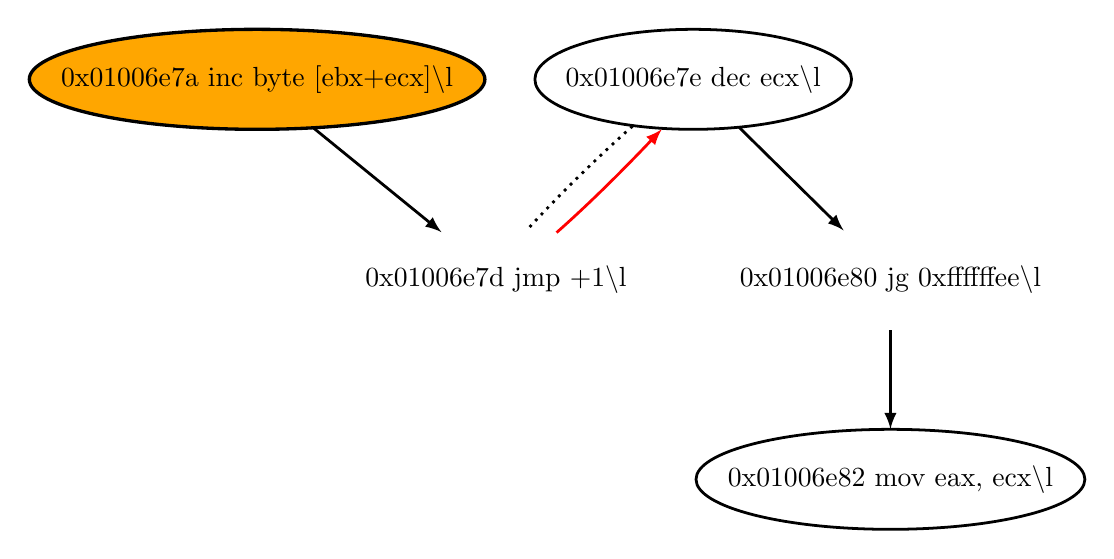
\begin{tikzpicture}[>=latex,line join=bevel,]
  \pgfsetlinewidth{1bp}
%%
\pgfsetcolor{black}
  % Edge: 0x0 -> 0x3
  \draw [->] (102.38bp,144.41bp) .. controls (113.79bp,135.12bp) and (128.17bp,123.42bp)  .. (148.36bp,106.99bp);
  % Edge: 0x4 -> 0x6
  \draw [->] (255.47bp,144.76bp) .. controls (264.48bp,135.88bp) and (275.81bp,124.71bp)  .. (293.13bp,107.63bp);
  % Edge: 0x4 -> 0x3
  \draw [dotted] (217.13bp,145.12bp) .. controls (204.55bp,133.98bp) and (189.45bp,119.13bp)  .. (179.17bp,107.8bp);
  % Edge: 0x3 -> 0x4
  \pgfsetcolor{red}
  \draw [->] (189.81bp,106.83bp) .. controls (199.7bp,115.58bp) and (211.16bp,126.64bp)  .. (227.69bp,144.05bp);
  % Edge: 0x6 -> 0x8
  \pgfsetcolor{black}
  \draw [->] (310bp,71.697bp) .. controls (310bp,63.983bp) and (310bp,54.712bp)  .. (310bp,36.104bp);
  % Node: 0x3
\begin{scope}
  \definecolor{strokecol}{rgb}{0.0,0.0,0.0};
  \pgfsetstrokecolor{strokecol}
  \draw (168bp,90bp) node {0x01006e7d jmp +1$\backslash$l};
\end{scope}
  % Node: 0x0
\begin{scope}
  \definecolor{strokecol}{rgb}{0.0,0.0,0.0};
  \pgfsetstrokecolor{strokecol}
  \definecolor{fillcol}{rgb}{1.0,0.65,0.0};
  \pgfsetfillcolor{fillcol}
  \filldraw [opacity=1] [very thick] (82bp,162bp) ellipse (82bp and 18bp);
  \draw (82bp,162bp) node {0x01006e7a inc byte [ebx+ecx]$\backslash$l};
\end{scope}
  % Node: 0x8
\begin{scope}
  \definecolor{strokecol}{rgb}{0.0,0.0,0.0};
  \pgfsetstrokecolor{strokecol}
  \draw (310bp,18bp) ellipse (70bp and 18bp);
  \draw (310bp,18bp) node {0x01006e82 mov eax, ecx$\backslash$l};
\end{scope}
  % Node: 0x6
\begin{scope}
  \definecolor{strokecol}{rgb}{0.0,0.0,0.0};
  \pgfsetstrokecolor{strokecol}
  \draw (310bp,90bp) node {0x01006e80 jg 0xffffffee$\backslash$l};
\end{scope}
  % Node: 0x4
\begin{scope}
  \definecolor{strokecol}{rgb}{0.0,0.0,0.0};
  \pgfsetstrokecolor{strokecol}
  \draw (239bp,162bp) ellipse (57bp and 18bp);
  \draw (239bp,162bp) node {0x01006e7e dec ecx$\backslash$l};
\end{scope}
%
\end{tikzpicture}

